\documentclass{beamer}
\usetheme{CMU}

\usepackage{pgf,pgfarrows,pgfnodes,pgfautomata,pgfheaps,pgfshade}
\usepackage{amsmath,amssymb}
\usepackage[utf8]{inputenc}
\usepackage{colortbl}
\usepackage[english]{babel}
\usepackage{booktabs}
\usepackage{slpython}
\usepackage{underscore}

\author{Luís Pedro Coelho}
\institute{Programming for Scientists}

\graphicspath{{figures/}{figures/generated/}{images/}}

\newcommand*{\code}[1]{\textsl{#1}}


\title{First Lecture: Course Policies and Course Overview}

\begin{document}

\section{Basics}
\frame{\maketitle}

\frame{\frametitle{Introduction}

\begin{block}{Who am I}
\begin{itemize}
\item Luís Pedro Coelho (lpc@cmu.edu)
\item Third year Ph.D.\ student in computational biology
\item My office is 409D, Mellon Institute
\end{itemize}
\end{block}

}

\frame{\frametitle{Introduction}

\begin{block}{This course}
\begin{itemize}
\item Meets: Tuesdays \& Thursdays 6.30pm 220 SH
\item Tuesday: Lecture
\item Thursday: Lab Session
\item Office Hours: Tuesday 5.30pm (or by appointment).
\item Course Website: http://coupland.cbi.cmu.edu/pfs
%\item Course Mailing List:
\end{itemize}
\end{block}

}
\frame{\frametitle{Homeworks}

There will be homeworks.
\note{
\begin{itemize}
\item Grades will depend on homeworks and final project.
\item Homeworks will be assigned on Tuesdays and are due the next Tuesday at mid-night.
\item Up to 24 hours delay: 20\% penalty. Up until beginning of lab-session: 30\% penalty.
\item Thursday sessions will often include discussion of homeworks, so after that, you can no longer turn in homeworks.
\item Homework will normally consists of a multiple-choice/short answer section plus a programming question.
\item Homeworks are to be turned in by email in text (.txt) or pdf format for the questions, and Python code for the programming (.py files).\\
    In particular, \textbf{doc, docx, odt} will not be accepted.
\end{itemize}
}

}

\frame{\frametitle{777 Rule}

\centering
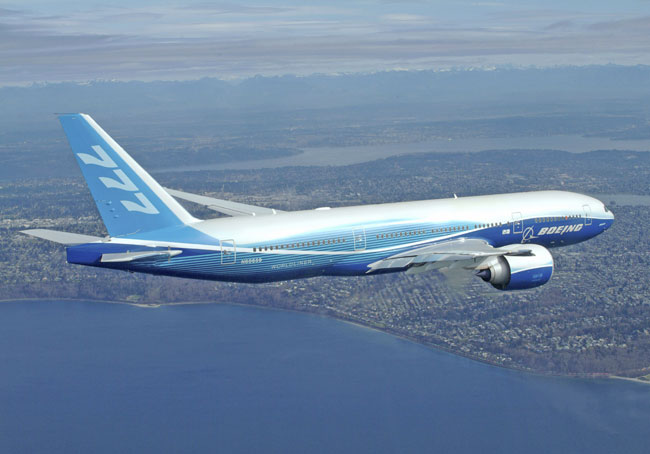
\includegraphics[width=.9\textwidth]{777}
% To pass: at least 7 (out of 10) on at least 7 homeworks, plus a 7 on the project

}

\frame{\frametitle{Project}

\begin{block}{Project}
\begin{itemize}
\item There will be a final project, which will replace homeworks towards the end of the class.
\item You can submit your own project, but I will have my own proposals.
\item You can work individually or in small groups. Expectations will scale linearly.
\end{itemize}
\end{block}
}

\frame{\frametitle{Course Structure}
\begin{block}{Two Lectures}
\begin{enumerate}
\item Tuesday session: a lecture where basic concepts are presented.
\item Tuesday session: a more lab type session, where we discuss particular technologies that let us implement the basic concepts.
\end{enumerate}
\end{block}

In fact, for the first module, the two sessions will resemble each other.
}
\section{Overview}
\frame{\frametitle{Programming for Scientists}

Programming\\
for\\
Scientists

}

\frame{\frametitle{Course Overview}
\begin{block}{Class Modules}
\begin{enumerate}
\item Structure of Programs
\item Basics of Scientific Programming
\item Advanced/Applied Topics
\end{enumerate}
\end{block}
}
\frame{\frametitle{Course Overview: Module I}

\begin{block}{Structure of Programs}
\begin{itemize}
\item Structured programming and general good programming
\item Object-based programming
\item Object-oriented programming
\end{itemize}
\end{block}
}
\frame{\frametitle{Basics of Scientific Programming}

\begin{block}{Scientific Programming}
\begin{enumerate}
\item Representation of numbers, memory usage
\item Numerical optimisation
\item Aspects of stochastic programming
\item Distribution of software
\end{enumerate}
\end{block}
}
\frame{\frametitle{Advanced Topics}

This is a mixed bag and subject to change (if you want to).

\begin{block}{Advanced Topics}
\begin{itemize}
\item Graphical user interfaces
\item Concurrent programming
\item Databases
\item Interfacing multiple languages (lab session only)
\end{itemize}
\end{block}
}
\section{Class Starts Here}

\begin{frame}[fragile]
Glass's Law 
\end{frame}

\begin{frame}[fragile]
\frametitle{Who Are Your Clients?}
\begin{block}{Different Classes of Users}
\begin{enumerate}
\item Other programmers (or you, next week).
\item Actual users (maybe you).
\end{enumerate}
\end{block}

In this class, we are focused on the programmers.
\end{frame}

\begin{frame}[fragile]

`` Programs must be written for people to read, and only incidentally for machines to execute.''
\begin{flushright}
---Abelson \& Sussman, \\\textit{Structure and Interpretation of Computer Programs}
\end{flushright}

\end{frame}

\frame{\frametitle{Principles of Good Code}

\begin{block}{Principles of Good Code}
\begin{itemize}
\item Correct
\item Sufficiently efficient
\item Robust
\item Readable
\item Tested
\item Extendable
\end{itemize}
\end{block}

}


\begin{frame}[fragile]
\frametitle{Code Organisation}

\begin{block}{Code Organisation}
The first section is on how to organise code.
\end{block}
\end{frame}

\begin{frame}[fragile]
\frametitle{Structured Programming}
\end{frame}

\begin{frame}[fragile]
\frametitle{A Bit of History}

\begin{block}{Programming Languages}
\begin{enumerate}
\item In the beginning, there was the bit.
\item Assembler
\item Fortran (1957, by \textsc{ibm})
\item Structured programming (late 60s). Algol 68, C, \ldots
\item Object-oriented programming. Simula, Smalltalk, C++, \ldots % FIXME
\end{enumerate}
\end{block}
\end{frame}

\begin{frame}[fragile]
\frametitle{Procedural Programming}
Procedural programming is code organised into procedures (functions).
\end{frame}

\begin{frame}[fragile]
\frametitle{Functions}
\begin{block}{A Good Function}
\begin{itemize}
\item Fits on the screen.
\item Has a small number of obligatory arguments.
\item Has a small number of outputs.
\item Can be tested separately from the rest of the program.
\end{itemize}
\end{block}
\end{frame}

\begin{frame}[fragile]
\begin{block}{Bad Code}
\begin{python}
def xyf(x,y):
    t=x*0.5
    t2=t/2
    t3=x*p
    t4=t2*t2-y
    t4=sqrt(t4)
    t5=t2-t4,t2+t4
    return t5

\end{python}
\end{block}
\end{frame}

\begin{frame}[fragile]

\begin{block}{Good Code}
\begin{python}
def quadratic_solution(a,b,c):
    '''
    xp, xm = quadratic_solution(a,b,c)

    Computes the two solutions to
        a * x**2 + b * x + c = 0
    '''
    Root = sqrt(b**2 - 4*a*c)
    x_plus = (-b + Root)/(2*a)
    x_minus = (-b - Root)/(2*a)
    return x_plus, x_minus

\end{python}

\end{block}
\end{frame}


\begin{frame}[fragile]
\frametitle{Good Variable Names}
\begin{block}{Principle}
Readibility
\end{block}
\begin{block}{Heuristics}
\begin{enumerate}
\item Don't be too short (except for $i$,$N$,\ldots)
\item Be conventional: loop iteration uses $i,j,k,\dots$, counts use $N$,\ldots
\item Try to avoid need for comments.
\item Exception: implementing code from a paper.
\end{enumerate}
\end{block}

\end{frame}

\begin{frame}[fragile]
\frametitle{Variable Name Examples}
\begin{python}
x = somefunction() # x represents the force
\end{python}

Why not?

\begin{python}
force = somefunction()
\end{python}

\end{frame}

\begin{frame}

%\includegraphics{}

\end{frame}

\begin{frame}[fragile]
\frametitle{Homework 0}

\begin{block}{Homework (for next week)}
Run the following Python program and email me the results:
\begin{python}
email="YOUR EMAIL"
print email, hash(email)
\end{python}
\end{block}
\end{frame}

\end{document}
